\chapter{Socio-Legal, Privacy, and Community Dynamics of Kernel-Level Anti-Cheat Implementations}
\label{annexe:one}

\fancyhead[LE]{\textsc{\chaptername~\thechapter}}

\section{System Visibility Level and Perceived Intrusion}

The architectural integration of anti-cheat software into the kernel layer shifts the boundaries of data access. Operating at Ring 0, a driver possesses the same execution privileges as the core operating system, effectively rendering the traditional memory protection boundaries of user-mode (Ring 3) obsolete.

\begin{itemize}
\item Theoretical Access to Non-Game-Related Data: Because kernel drivers have unrestricted access to the entire Virtual Address Space, they can theoretically read and monitor memory pages belonging to unrelated applications. This includes open web browsers containing active sessions, password managers, encryption keys, and local files. While publishers assert that their drivers only scan for cheat signatures, the technical capability to perform deep packet and memory inspection across the entire system remains a valid point of concern for privacy advocates.
\item Continuous vs. Occasional Monitoring: A major shift occurred with the introduction of Riot Games' Vanguard (vgk.sys), which mandates an "always-on" approach. Unlike traditional anti-cheats that initialize alongside the game client and terminate upon closure, always-on kernel drivers boot during the system startup sequence. The industry justification is to prevent the pre-loading of cheats or hypervisors before the anti-cheat can initialize. However, this creates a state of continuous monitoring, leaving a privileged third-party component active even when the user is performing sensitive tasks unrelated to gaming.
\item The Notion of Implicit Consent: End-User License Agreements (EULAs) operate on a
"take-it-or-leave-it" basis. Users are faced with a asymmetric choice: surrender Ring 0 access to their personal computer or lose access to the digital service entirely. In academic literature, this undermines the principle of freely given and informed consent, as the economic and social pressure to maintain connection with peer groups in modern video games forces users to accept invasive telemetric conditions.
\end{itemize}

\section{Social Perception and Community Acceptance}

The deployment of kernel-level anti-cheats has transformed a purely technical challenge into a highly polarized cultural debate within the global gaming community.

\begin{figure}[H]
    \begin{center}
        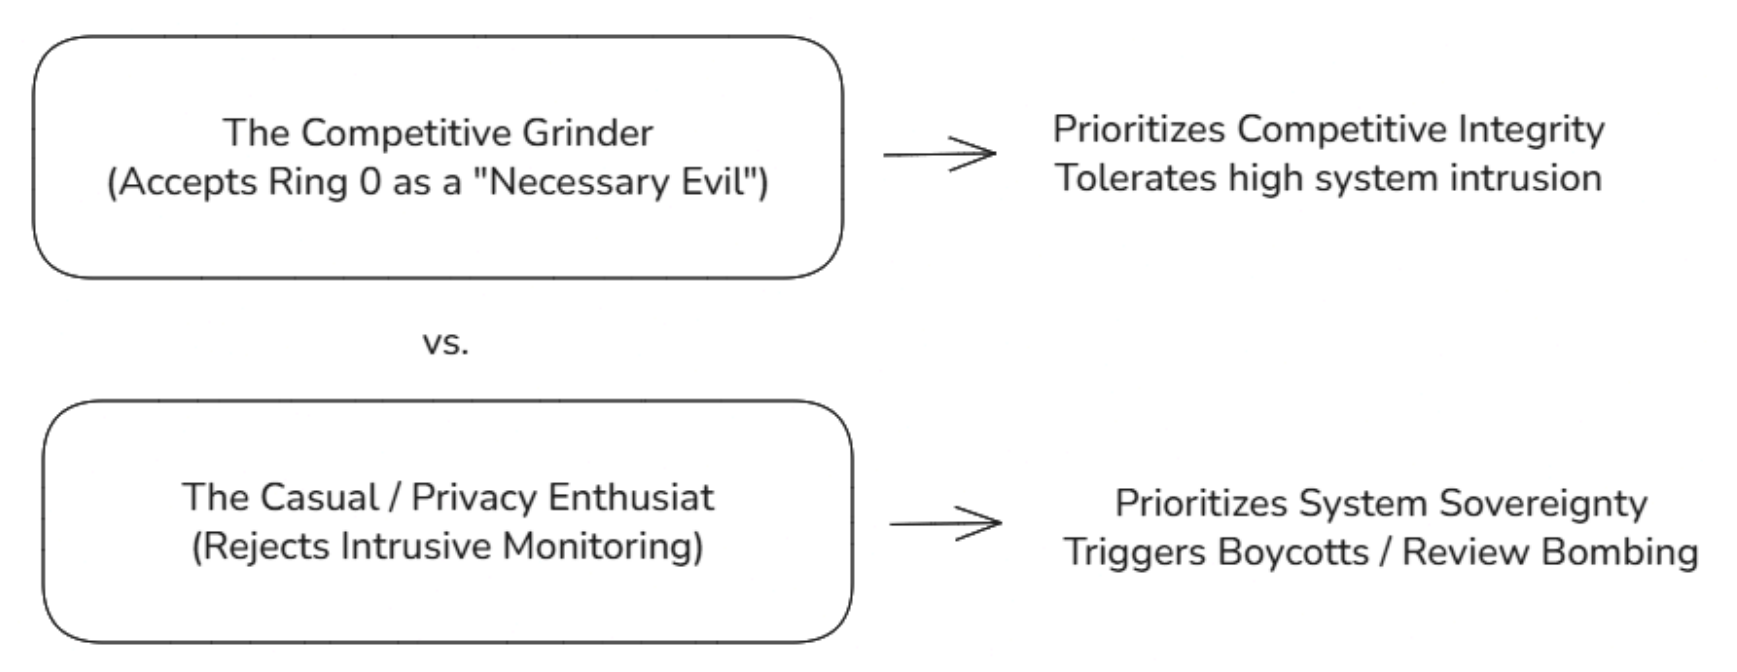
\includegraphics[width=15cm]{../images/annex01/fig6.png}
    \end{center}
    \caption{User Segmentation \& Acceptance Divide}
    \label{fig:fig6}
\end{figure}

\begin{itemize}
\item Public Debates Around Intrusive Anti-Cheats: High-profile releases have frequently triggered severe community backlash. For example, the launch of Helldivers 2 faced significant criticism and review-bombing on platforms like Steam due to its implementation of nProtect GameGuard. Users frequently cite performance degradation, potential system instability, and the lack of transparency regarding what data is transmitted back to external servers as primary grievances.
\item The Divide Between Competitive and Casual Players: The player base is structurally divided regarding acceptability. Highly competitive players, particularly within esports ecosystems, often champion intrusive client-side measures, viewing them as a necessary tool to safeguard competitive integrity and financial stakes. Conversely, casual players or hardware enthusiasts view these measures as disproportionate. This divide is further amplified by ecosystem fragmentation, such as the complete exclusion of Linux and Steam Deck users from titles like League of Legends or Apex Legends due to the technical incompatibility of kernel drivers with translation layers like Proton.
\item Impact on Game Adoption: This friction directly impacts the commercial viability of software. A growing segment of privacy-conscious consumers actively boycotts games utilizing kernel-level solutions. For publishers, this creates an operational trade-off: mitigating financial losses caused by cheaters versus losing potential customers who refuse to compromise their system sovereignty.
\end{itemize}

\section{Legal and Regulatory Questions}

From a legal perspective, the deep monitoring required by client-side kernel components tests the boundaries of modern data protection frameworks and civil liability.

\begin{itemize}
\item GDPR Compliance: Proportionality and Data Minimization: Under Article 5(1)(c) of the General Data Protection Regulation (GDPR), personal data processing must be adequate, relevant, and limited to what is necessary in relation to the purposes for which they are processed (data minimization). Proving that an anti-cheat requires sweeping visibility over a user's entire operating system to catch cheaters represents a precarious legal position. If a server-side or behavioral approach can achieve similar outcomes without local system surveillance, the kernel-level approach may fail the core GDPR test of proportionality.
\item Liability in Case of a Security Flaw: Standard EULAs explicitly disclaim all corporate liability for software-induced damages, hardware conflicts, or data breaches. However, from a consumer rights perspective, the mandatory installation of a software component capable of creating an exploitable system vulnerability (e.g., the historical Capcom driver exploit or the Genshin Impact anti-cheat exploit used to deploy ransomware) challenges these liability waivers. Should a major anti-cheat driver be weaponized on a global scale, publishers could face unprecedented class-action lawsuits concerning negligence in secure software design.
\item Transparency and Terms of Service: Most publishers offer limited visibility into the telemetry data collected by their kernel components. The lack of open-source auditing or independent third-party verification means users must blindly trust corporate assertions. To align with modern transparency mandates, anti-cheat developers face growing pressure to provide detailed documentation, open APIs, or clear, granular logs showing precisely what memory segments are being analyzed and when data is being exfiltrated to the cloud.
\end{itemize}